\chapter{Stationary properties} 


\section{Boundary conditions}

To obtain the spectrum of the system it's necessary to find the boundary conditions. As the barrier chemical potential  is the biggest energy parameter of the problem, the wave-functions there are defined by the Hamiltonian:
\begin{gather}
\label{barrier_Hamiltonian}
	H(y)
	=
	\br{
		\frac{p^2}{2m}
		+\mu_b
	}\tau_z,  ~~~~~~~~~-\frac{L}{2}<y<\frac{L}{2}
\end{gather} 

as the low energies are the under consideration, in Sroedinger equation the energy term can be omitted, so $ p_b\approx\pm i \sqrt{2m\mu_b} $. One can solve the problem given by (\ref{barrier_Hamiltonian}) and match the values of the wavefunction and it's derivatives on the left and on the right of the barrier to obtain:
\begin{gather}
	\begin{cases}
	\psi_L + b\partial_y\psi_L=t(\psi_R + b\partial_y\psi_R) \\
	\psi_R - b\partial_y\psi_R=t(\psi_L - b\partial_y\psi_L)
	\end{cases}
\end{gather}

here $ \psi_{L,R}=\psi\br{\mp\frac{L}{2}} $, $ b=\br{{2m\mu_b}}^{-\frac{1}{2}} $ --- the penetration depth for the particle inside th barrier and $ t = e^{-\frac{L}{b} }$ --- the tunneling constant assumed to be small: $ t\ll 1 $. This condition reads, that the size of the barrier $ L $ should be  much bigger that the penetration depth $ b $.

This condition is invariant under the combined action $ L\leftrightarrow R $, $ y\to-y $. To simplify the further analysis one can reverce th direction in the left wire and put both ands of the wires from $ y= \frac{L}{2} $ to $ y=0 $. The boundary condition than becomes:
\begin{gather}
\label{bc_transformed}
\begin{cases}
\psi_L - b\partial_y\psi_L=t(\psi_R + b\partial_y\psi_R) \\
\psi_R - b\partial_y\psi_R=t(\psi_L + b\partial_y\psi_L)
\end{cases}
\end{gather}
This transformation is illustrated on the fig \ref{fig:bctransform}.

The boundary condition (\ref{bc_transformed}) can be rewritten with introducing the spinor $ \Psi=\br{\psi_L, \psi_R}^T $ and Pauli matrices $ s_i $ in LR space:
\begin{gather}
	\br{1-ts_x}\Psi-\br{1+t s_x}b\pdy\Psi=0
\end{gather}
since for all $ t\ne 1 $ (recall, that $ t\ll1 $) the matrix is $ 1\pm ts_x $ in reversible. Multupliing the last equation by $ \br{1-ts_x}/\br{1+t^2} $ one obtain:
\begin{gather}
\label{bc_LR_space}
	\br{1-2\tilde{t}-\tilde{b}\pdy}\psi=0
\end{gather}
where $ \tilde{t}=\frac{t}{1+t^2} $, $ \tilde{b} = \frac{1-t^2}{1+t^2}b $. In the leading order on $ t $, which corresponds to the tunneling limit, $ \tilde{t}=t $, $ \tilde{b} = b $.
\begin{figure}[H]
	\centering
	\includegraphics[width=0.9\linewidth]{images/bc_transform}
	\caption{Illustration of switching the direction of left wire}
	\label{fig:bctransform}
\end{figure}

One can argue, that in tunneling limit the second and the third term in (\ref{bc_LR_space}) are much smaller than the first one and should not be taken when the leading order is considered. However, if the second terms is omitted, the leads become efficiently disconnected, and no tunnel effects can be found. The same is true for the third term --- if it's not present, the boundary condition immediately implies $ \Psi\br{0} = 0 $, so the wires become disconnected again.

\section{High momentum modes}  

As was pointed in section \ref{sec:high_and_low_modes}, there are two  shortwave and longwave wavefunctions inside the wire, and the first ones can be described with the Hamiltonian (\ref{short-long_hamiltonian}). However, if one is looking for the localized states, even the longwave modes should be taken decaying. To obtain this, one needs to add a restore superconducting term in (\ref{short-long_hamiltonian}), so the spectrum become gapped and the momenta can get an imaginary part. So, for shortwave modes one should consider a Hamiltonian:
\begin{gather}
\label{high_mods_hamiltonian}
	H=\br{\frac{p^2}{2m}-ups_z\sigma_z}\tau_z+\Delta\tau_\phi
\end{gather}
here the multiplier $ s_z $ is added in the spin-orbit coupling term, as the direction of the left wire is inverted, so to write a correct Hamiltonian for LR space, one needs to change $ p $ to $ -p $ for the left wire --- which is exactly adding $ -s_z $ multiplier to each momentum.

Denoting $ \eta = \frac{p^2}{2m}-ups_z\sigma_z $, one can rewrite (\ref{high_mods_hamiltonian}) as $ H=\eta\tau_z+\Delta\tau_\phi $. As $ s_z\sigma_z $ commutes with $ H $ one can treat it as a number, so the dispersion is $ E^2 =\eta^2+\Delta^2 $. Thus $ \eta=\pm i\sqrt{\Delta^2-E^2} $, as the case $ \abs{E}<\Delta $ is assumed. For shortwave one can write the equation:
\begin{gather}
	p^2-2mu s_z \sigma_z p - 2m \eta =0
\end{gather}
which for shortwave momenta gives $ p_{short}\approx2 mu s_z \sigma_z + \frac{\eta}{u}s_z\sigma_z$. Choosing the sign of $ \eta $ in a way, that the wavefunction decays at $ x\to \infty $, one can obtain:
\begin{gather}
\label{short_momentum_decaying}
	p_{short}\approx
	2 mu s_z \sigma_z 
	+
	i\frac{\sqrt{\Delta^2-E^2}}{u}
\end{gather}


Now the wavefunction can be constructed by putting (\ref{short_momentum_decaying}) into the Schroedinger equation $ \br{\eta\tau_z +\Delta\tau_\phi}\Psi=E\Psi $. The solutions are:
\begin{gather}
	\Psi_{s_z,\sigma_z}\br{x}
	=
	\begin{pmatrix}
	1
	\\
	e^{i\br{s_z\sigma_z\gamma+\phi_{s_z}}}
	\end{pmatrix}_{eh}
	e^{2imus_z\sigma_zx -\frac{\sqrt{\Delta^2-E^2}}{u}x}
	\ket{s_z, \sigma_z}
\end{gather}
where $ s_z $ and $ \sigma_z $
 should be treated as numbers can be equal $ \pm1 $, $ \ket{s_z, \sigma_z} $ are eigenvectors of matrix $ s_z \sigma_z $ and $ \gamma = -\frac{\pi}{2}+\arcsin\frac{E}{\Delta} $.
Thus the longwave part of eqigenstate can be written as:
\begin{gather}
	\Psi_{long}
	=
	\sum_{s_z=\pm 1}
	\sum_{\sigma_z=\pm 1}
	\Psi_{s_z,\sigma_z}\br{x}
\end{gather}
 
  \if 0
\begin{gather}
\begin{pmatrix}
i s_z \sigma_z\sqrt{\Delta^2-E^2}-E & \Delta e^{-i\phi_{L,R} s_z} \\
\Delta e^{i\phi_{L,R} s_z} & -i s_z \sigma_z\sqrt{\Delta^2-E^2}-E
\end{pmatrix}
\Psi
=
E\Psi
\end{gather}
\fi
and